\section{Претрага Интернета и обрада хипервеза}

\subsection{Проналажење информација}

Проналажење информација\index{pronalazenje informacija@проналажење информација} може се дефинисати као процес претраживања унутар неког документа и/или колекције докумената за потребном информацијом\cite{langville2011google}. Кроз историју се проблем проналажења информација у документима почео решавати још у 5. веку п.н.е. у Античкој Грчкој, кад је први пут уведен \emph{садржај} у неки од свитака папируса, пошто књиге у данашњем облику тада још нису постојале. У Старом Риму проблем су решавали етикетама налик на данашње \emph{Post-it} налепнице. Све се, наравно, променило са проналаском штампарске машине, средином 15. века. Крајем 19.века почиње да се имплементира Дјуијев\index{Djui@Дјуи} децимални систем\footnote{Dewey, 1872. Сортирао је колекције према тематици, на пример, троцифреним бројевима који почињу са 1 је означавао филозофију, са 2 религију, итд. Тако да је, на пример, књига са идентификационим бројем 142 означавала књигу о филозофији.}, каталог картица. У 20. веку долази до употребе технологије у претраживању докумената, па се тако појављују микрофилмови. У '60-им годинама прошлог века направљена је прва машина која је радила претрагу информација, а ради се о \emph{MARC}\footnote{енгл., \emph{Machine Reading Catalog}}\index{MARC@\emph{MARC}} рачунару. Данас се у традиционалном претраживању\index{tradicionalno pretrazivanje@традиционално претраживање} и проналажењу информација користи систем картица (на пример у библиотекама), али доминирају компјутерски помогнути системи. У овим последњим постоје три карактеристична модела за претраживање: \emph{буловски}, \emph{векторски}, \emph{модели вероватноће}\cite[Ch 1.2]{langville2011google}. Постоји на хиљаде модела, али су сви настали као варијанте три горе наведена.

\textbf{Буловски модел}\index{tradicionalno pretrazivanje@традиционално претраживање!Bulovski model@Буловски модел} користи систем егзактног подударања да нађе документ који корисник захтева. Име је добио по Буловој алгебри, чије логичке операторе користи. Не постоји концепт парцијалног подударања што је велики проблем, ако је потребно да пронаћи документ, за који се не зна тачан назив. Проблеми претраживања информација, као што су проблем синонима и проблем вишезначности, овде се не могу избећи.

\textbf{Векторски модел}\index{tradicionalno pretrazivanje@традиционално претраживање!Vektorski model@Векторски модел} је увео Џералд Салтон,'60-их година прошлог века. Базира се на трансформацији текстуалних података у нумеричке векторе и матрице и примењује се матрична анализа за откривање повезаности кључних речи. Овакви модели решавају проблеме синонима и вишезначности. Резултати се могу презентовати сортирани према степену релевантности.\cite{berry2005understanding}

\textbf{Модели вероватноће}\index{tradicionalno pretrazivanje@традиционално претраживање!Modeli verovatnoce@Модели вероватноће} покушавају да процене вероватноћу којом ће корисник наћи жељени документ у односу на упит. Резултати се могу поређати по изгледима релевантности. Треба истаћи да није једноставно имплементирати овакве моделе у рачунарско окружење.\cite{berry2005understanding}

\subsection{Проналажење информација на вебу}
Када је у марту 1989. године британски инжењер Тим Бернерс-Ли\index{Tim Berners Lee} послао предлог\cite{proposal} да се унапреди информациони систем у \emph{CERN}-у\footnote{Европска организација за нуклеарна истраживања (франц., \emph{Conseil Européen pour la Recherche Nucléaire})}\index{CERN@\emph{CERN}}, није ни слутио у шта ће се претворити једноставна потреба за хипервезивањем основних података о запосленим у \emph{CERN}-овом информационом систему\cite{berners2004weaving}. Тим Бернерс-Ли је за потребе новог информационог система измислио нови језик који је назвао \emph{Hypertext Markup Language}\index{HTML@\emph{HTML}}, одн. \textbf{HTML}.

Од прве веб странице из маја 1990. године до данас је прошло више од 20 година, а у овом тренутку постоји неколико милијарди веб страница. Јасна је мотивација која се од почетка јавила корисницима веба, а то је како наћи праву информацију. Веб\index{veb@веб} је огроман, динамичан, самоорганизован и хиперповезан.\cite[Ch 1.3.1]{langville2011google} Свако може поставити веб страницу\index{veb@веб!veb stranice@веб странице}. Странице се мењају дневно, па чак и чешће. Нове странице се појављују сваки минут. То су реални проблеми веб претраживања, на које није могло да одговоро традиционално претраживање информација. Такође, корисници ретко погледају више од 10 до 20 докумената који су понуђени, што појачава потребу да резултати морају бити јако прецизни и брзо достављени кориснику.

Први Интернет претраживач је био \emph{Archie}\index{Archie@\emph{Archie}}, направљен 1990. године, од стране канадског студента Алана Емтејџа. Примарни протокол је био \emph{ftp}. Први робот\index{robot@робот} који је аутоматски индексирао странице звао се \emph{World Wide Web Wanderer} који је своје резултате стављао у прву базу хипервеза веб страница \emph{Wandex}\index{robot@робот!Wandex@\emph{Wandex}}. До средине '90-их направљено је на хиљаде \emph{веб-паукова} тј. робота који су складиштили информације са веба. На жалост, ти веб-паукови нису знали како да искористе те информације на добар начин. 1994. године појавио се \emph{Yahoo}\index{veb pretrazivac@веб претраживач!Yahoo@\emph{Yahoo}} као збир неколико популарних страница и са директоријумом популарних страница. У том тренутку \emph{Yahoo} се не може сматрати претраживачем. Али 1994. године се појављују два значајна \emph{веб-паука}\index{crawler@\emph{crawler}}-а, \emph{WebCrawler}\index{crawler@\emph{crawler}!WebCrawler@\emph{WebCrawler}} и \emph{Lycos}\index{crawler@\emph{crawler}!Lycos@\emph{Lycos}}, чији се број сакупљених хипервеза мерио у десетинама милиона. У децембру 1995. године појављује се први прави веб претраживач\index{veb pretrazivac@веб претраживач} \emph{AltaVista}\index{veb pretrazivac@веб претраживач!AltaVista@\emph{AltaVista}} који је омогућавао примену логичких оператора. \emph{AltaVista} је користила, из данашњег угла гледања врло лош алгоритам рангирања страница, који се заснивао на провери тзв. мета-података из заглавља HTML документа и врло лако је могао да се злоупотреби и зато је пројекат пропао крајем 20. века. Са појавом \emph{Google}-а\index{veb pretrazivac@веб претраживач!Google@\emph{Google}}, тј. његовог претраживача, веб претраживач \emph{AltaVista} долази у озбиљне проблеме.

Два су кључна алгоритма за даљи развој веб претраживања: \emph{PageRank}\index{PageRank@\emph{PageRank}} и \emph{HITS}\index{HITS@\emph{HITS}}. Први је омогућио Гуглу да постане оно што данас јесте -најкоришћенији претраживач са највише индексираних страница, док је \emph{HITS} дело Џона Клајнберга из IBM-а купљен од стране \emph{Тeome}, данашњег \texttt{ask.com}. Оба алгоритма су се јавила независно један од другог исте, 1998. године. Више о PageRank алгоритму у даљем делу рада.

\subsection{Процес веб претраживања}\label{subsec:web}

Веб претраживач\index{veb pretrazivac@веб претраживач} је веб апликација која ће претражити веб странице, извући све могуће хиперлинкове, рангирати их и на крају дати најбоље могуће решење за задату кључну реч. Апликација се састоји из више елемената:

\begin{itemize}
\item модул веб-паука
\item модул индексизације
\item индекс
      \begin{itemize}
      \item индекс садржаја
      \item индекс структуре
      \item индекс за специјалне сврхе
      \end{itemize}
\item складиште страница
\item модул упита
\item модул рангирања
\end{itemize}

Процес се састоји од узајамног деловања претходно набројаних модула. Тако веб-паук скупља странице по вебу, целе странице одлаже у \emph{складиште веб страница}, док хипервезе шаље у индекс, који их поставља уз кључне речи које добија из модула индексовања. Кад корисник пошаље упит, модул упита тражи од индекса скуп свих решења, која се кроз модул рангирања на крају постављају као резултати корисниковог упита. Модел процеса може се представити као што је то урађено на слици  \ref{slike:crawling}.

\begin{figure}
\centering
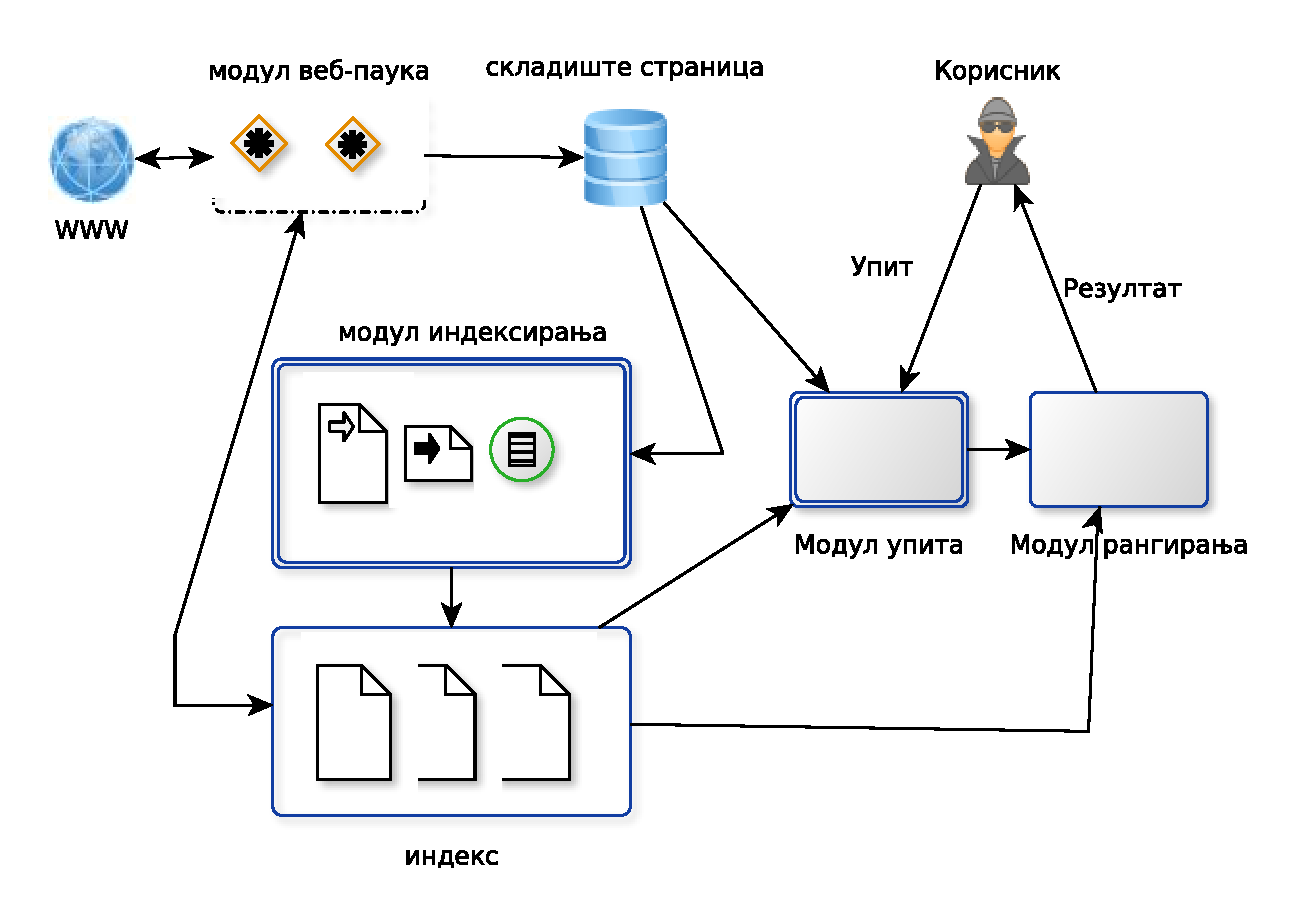
\includegraphics[scale=0.5]{crawler.eps}
\caption{Процес веб претраживања \cite[Ch 1.3.2]{langville2011google}}
\label{slike:crawling}
\end{figure}

\subsection{Извлачење хипервезе}

У процесу реализације к\^{о}да веб претраживача, прво је потребно написати програм веб-паука, који ће претражити страницу и наћи прво један, па онда и све остале хипервезе. Да би се пронашла хипервеза, потребно је знати како изгледа веб страница.

\subsubsection{Структура HTML странице}
Веб страница\index{HTML@\emph{HTML}}\index{veb@веб!veb stranice@веб странице} је заправо само дугачак низ знакова који образују HTML к\^{о}д. Веб прегледач претвара к\^{о}д у изглед који се обично добија на екрану приликом избора неке странице. Да би се видео дати к\^{о}д који генерише веб страницу,  зависно од веб прегледача који се користи (\emph{Internet Explorer}, \emph{Firefox}, \emph{Safari} или \emph{Chrome}, на пример), потребно је потражити опцију ,,View Page Source'', ,,View Source'' или слично.

Структура овог рада не омогућава претерано улажење у HTML\index{HTML@\emph{HTML}}, те ће се упрошћено навести како изгледа структура HTML к\^{о}да\cite{strukturaHTML}. Дакле, структура веб стране је следећа:

\begin{itemize}
\item <html> таг;
\item Заглавље, у којем се налазе подаци о наслову странице, аутору, разним  мета подацима везаним за страницу и све то се налази између <head> и </head> ознака;
\item Садржај странице, који се исписује између <body> и </body> ознака;
\item затвара се </html> ознаком
\end{itemize}

Интересантно за овај рад је како су означене хипервезе у том к\^{o}ду.

\subsubsection{HTML <a> tag}
За веб-паука од највеће важности је пронаћи хипервезе ка другим  веб страницама. Хипервезе у HTML\index{HTML@\emph{HTML}!a@<a>} к\^{о}ду се налазе унутар <а> ознаке. Наиме, хипервеза се задаје на следећи начин:

\begin{lstlisting}[caption = <a> ознака, label = a_tag]
<a href="<url>">
<a href="http://www.matf.bg.ac.rs">
\end{lstlisting}

Дакле, да би се пронашла хипервеза унутар HTML к\^{о}да, потребно је прво пронаћи <a> ознака.

\subsubsection{Налажење првог хиперлинка}

Алгоритам за налажење прве хипервезе\index{HTML@\emph{HTML}!hiperlink@хиперлинк} у HTML к\^{о}ду, почиње од налажења <a href=" дела, а сама хипервеза ће се наћи између знакова навода који следе после горе поменутог дела HTML тага. Следи к\^{о}д који то успешно ради:

\begin{lstlisting}[caption = Налажење првог хиперлинка, label = {lst:first_url}, numbers = left]
# u promenljivoj page je smestena niska celog
# HTML koda internet stranice
page = '<sadrzaj veb stranice>'

# trazi se prvo pojavljivanje <a> oznake i
# smesta se u promenljivu start_link
start_link = page.find('<a href=')

# trazi se prvo pojavljivanje znaka navoda
start_quote = page.find('"', start_link)
# trazi se zatvaranje navodnika
end_quote = page.find('"', start_link+1)
# hiperveza je sve izmedju dva znaka navoda
url = page[start_quote + 1 : end_quote]
\end{lstlisting}

\subsection{Налажење свих хипервеза на страници}

Да би се пронашле и остале хипервезе потребно је да наставити са претходно описаним процесом тражења хипервезе. Ради тога, уводи се процедура која ће омогућити налажење следеће хипервезе.

\subsubsection{Процедура трагања за следећом хипервезом}

Да би се пронашла прва следећа хипервеза, односно да би се установило где ће бити почетак следеће хипервезе, потребно је пронаћи следећу <а> ознаку и тада поновити к\^{о}д за налажење прве хипервезе. Та процедура би требало да изгледа овако:

\begin{lstlisting}[caption= Процедура налажења прве следеће хипервезе, label={lst:get_next_target_1}, numbers = left]
def get_next_target (page):
    start_link = page.find('<a href=')
    start_quote = page.find('"', start_link)
    end_quote = page.find('"', start_quote+1)
    url = page[start_quote+1:end_quote]
    return url, end_quote
\end{lstlisting}

Oвa процедурa враћa вредност хипервезе коју је пронашла, али и позицију завршног знака навода, како би се знало где је стала процедура и наставило са тражењем осталих хипервеза.

\subsubsection{Ако нема линкова?}

Потребно је решити проблем са горе поменутом процедуром у ситуацији да нема хипервеза у страници. Решење је да се постави услов, ако се не нађе почетак хипервезе, онда се враћа кључна реч \lstinline{None}, која означава празну ниску.

\begin{lstlisting}[caption = Испитивање да ли страница садржи хипервезу, label={lst:get_next_target_2}, numbers = left]
def get_next_target (page):
    start_link = page.find('<a href=')
    if start_link == -1:
        return None, 0
    start_quote = page.find('"', start_link)
    end_quote = page.find('"', start_quote+1)
    url = page[start_quote+1:end_quote]
    return url, end_quote
\end{lstlisting}

За испитивање у услову је коришћена вредност -1, јер Python враћа ту вредност ако не нађе задату ниску, тј. ако ниска не постоји.

\subsubsection{Све хипервезе}		Сад је могуће, користећи процедуру get\_next\_target(в. к\^{о}д \ref{lst:get_next_target_2}), одштампати све хипервезе\index{HTML@\emph{HTML}!hiperlink@хиперлинк} једне веб странице. Претпоставља се да је у променљивој \emph{page}, смештен HTML к\^{о}д неке веб странице.

\begin{lstlisting}[caption=Процедура штампања свих хипервеза, label={lst:print_all_links}, numbers = left	]
def print_all_pages(page):
    while True:
         url, endpos = get_next_target(page)
         if url:
             print url
             page = page[endpos:]
         else:
             break
\end{lstlisting}

У претходном коду користи се ,,\lstinline{while True}'', пошто је потребно налазити нове хипервезе све док их има на страници, а ако их нема, наредбом \lstinline{break} излази се из петље.
